% created on 2021-02-09
% @author : Zacharias Chalampalakis 
\chapter{Introduction to PET imaging and Pharmacokinetic modelling}

Positron emission tomography (PET) is a quantitative imaging technique that makes use of 
positron-emitting radioisotopes for the study of biochemical and physiological processes \textit{in vivo}. The molecules of interest for the studies processes are labelled with a radioisotope and then introduced in the body. The PET imaging system is used to collect information about the location of the labelled molecules \textit{in vivo} and create a map of activity distribution. Information can be collected dynamically over time to track distribution changes with time and deduce information for the characterisation of the underlying process kinetics. 
\section{Principles of PET}


\section{Principles of pharmacokinetic modelling }
Pharmacokinetics refers to the study of absorption, distribution, metabolism and excretion of drugs in living systems. The study of pharmacokinetics is based on measurements of concretion of drugs and their metabolites in the body over time. Mathematical relationships can be derived in order to study the 

\begin{figure}[ht]
	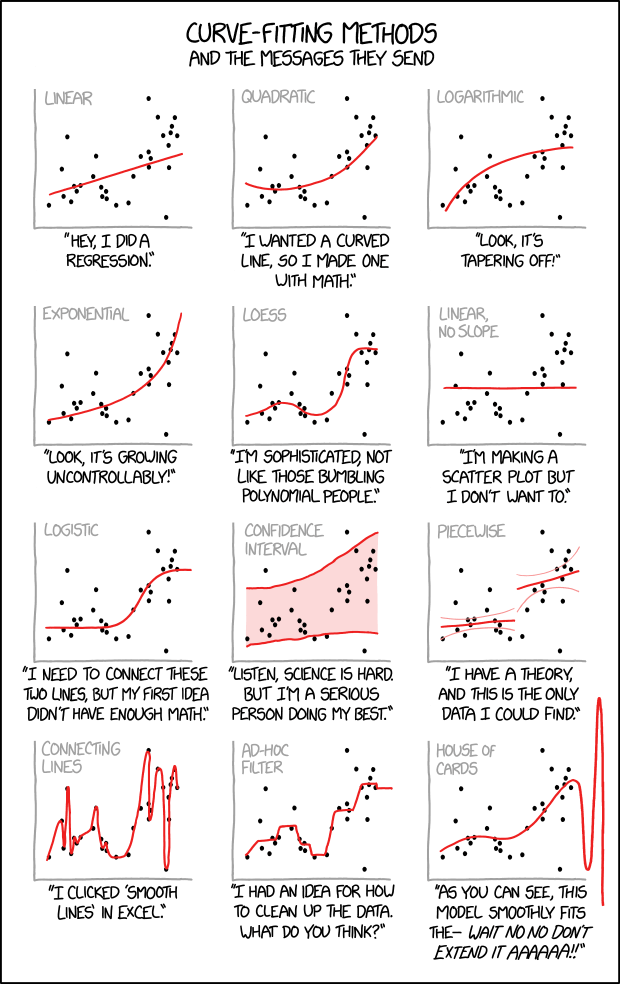
\includegraphics[width=0.8\textwidth]{figures/curve_fitting}
	\centering
	\caption{Important graphs for my research.}
	\centering
	\label{fig:curve_fitting}
\end{figure}